\subsection{RSS3 \glsfmtfull{GI}}
\label{subsec:GI}

{
    \begin{figure}[tb!]
        \centering
        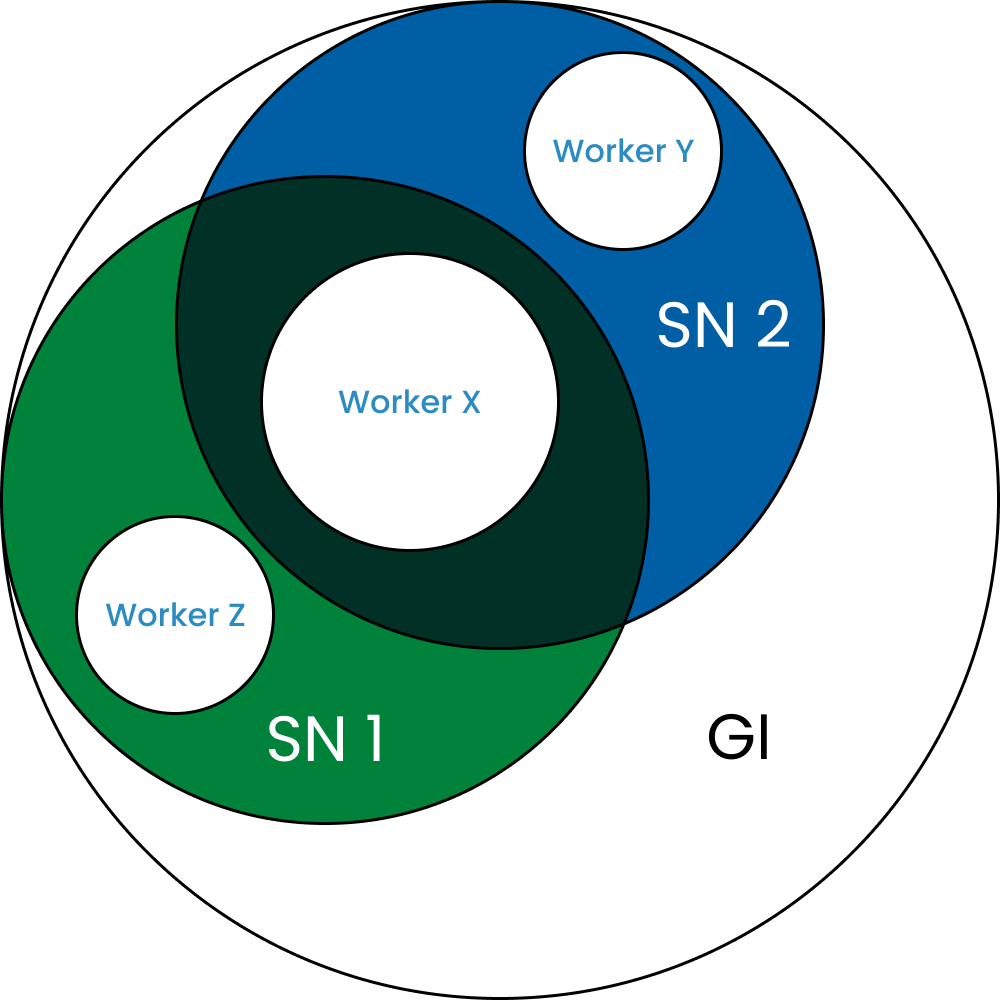
\includegraphics[width=0.8\columnwidth]{figures/GI.png}
        \caption{A Venn diagram illustrating the relationship between the worker, the \glsfmtlong{Node}, and the \glsfmtlong{GI}.}
        \label{fig:GI}
    \end{figure}
}

\glspl{GI} are responsible for facilitating coordination among \glspl{Node} and engaging with the \gls{VSL} and perform critical duties via the contracts \cite{settlementcontract,stakingcontract,networkparamscontract} to ensure the \gls{DSL} is robust and reliable.
The source code is openly available \cite{rss3globalindexer}.

Given the permissionless nature of the \gls{DSL}, robust quality assurance is essential to maintain the integrity and reliability of the \glsfmtlong{R3N}.
As such, the operation of a \gls{GI} is subject to a set of stringent requirements imposed by the Network.

{
    \begin{figure}[tb!]
        \centering
        \includegraphics[width=0.8\columnwidth]{figures/GI-components.png}
        \caption{Components of a \gls{GI}. See \Cref{subsec:GI} for more details.}
        \label{fig:GI-components}
    \end{figure}
}

Each \gls{GI} is composed of several components, each with a unique set of responsibilities and functions that collectively contribute to the overall reliability and robustness of the \gls{DSL}.

\subsubsection{Broadcaster}
The broadcaster is a component that continuously monitors all \glspl{Node} to detect any unusual or unexpected behavior.

\subsubsection{Enforcer}
The enforcer maintains demotion and slashing records, and implements measures to encourage \glspl{Node} to meet the established requirements.

\subsubsection{Indexer}
The indexer component provides structured information through its network transparency API, offering comprehensive insight into Network operations.

\subsubsection{Payment Processor}
The payment processor collects request fees from requesters.
In addition, it calculates the Network's average tax rate and updates the settlement contract on the \gls{VSL} accordingly.

\subsubsection{Router}
The router is responsible for routing requests to corresponding \gls{Node} with optimal performance and minimal latency.
The distinctive architecture of the \gls{DSL} requires \glspl{GI} be equipped with enhanced computational capabilities to determine the most efficient routing path for incoming requests.
Typically, a request retrieves \glsfmtlong{OI} from a distributed group of \glspl{Node} concurrently.

\subsubsection{Settler}
The settler component submits \glspl{Node}' work records to the \gls{VSL}. Subsequently, the settlement contract on the \gls{VSL} verifies these records and facilitates the distribution of network rewards.

\subsection{Reliability Score}

A \gls{GI} routes requests to \glspl{Node} based on their information coverage and a \gls{RS}.
The calculation of \reliabilityScore\ is based on a range of factors, including but not limited to the \gls{Node}'s uptime, work, slash records, operation deposit, and staking/trust pool size.
\glspl{Node} with a higher \reliabilityScore\ have an increased likelihood of receiving requests.